\section*{Informations générales}
 
\begin{table}[H]
\centering
	\begin{tabularx}{16.8cm}{|X|X|}
	\hline
	\rowcolor{gray!40} Numéro du risque & Type du risque \\
	\hline
	009 & Absence de serveur extérieur \\
	\hline
	\end{tabularx}
\end{table}

\begin{table}[H]
\centering
	\begin{tabularx}{16.8cm}{|X|X|X|}
	\hline
	\rowcolor{gray!40} Date & Visa du \RQ & Visa du \CP \\
	\hline
	 28/01/2016 & pgpic & pgpic \\
	\hline
	\end{tabularx}
\end{table}

\begin{table}[H]
\centering
	\begin{tabularx}{16.8cm}{|X|X|X|X|}
	\hline
	\rowcolor{gray!40} Pilote & Activité WBS & Compte WBS & Phase d'apparition \\
	\hline
	 \Matthieu & Suivre les Risques et Opportunités & 1.2.3.2 & À partir du début du projet\\
	\hline
	\end{tabularx}
\end{table}

\section*{Description du risque}

\subsection*{Résumé}
	Le risque lié à l'absence de serveur gratuit pour déployer notre livrable nous obligerait à nous retourner vers une solution payante qui ne satisferait pas le client.
	
\subsection*{Analyse des causes}
	voir figure \ref{risque pas de serveur ext}.

\subsection*{Criticité}

\begin{table}[H]
\centering
	\begin{tabularx}{16.8cm}{|>{\columncolor{gray!40}}X|X|}
	\hline
	Gravité & 4\\
	\hline
	Probabilité & 4\\
	\hline
	Criticité & Critique\\
	\hline
	\end{tabularx}
\end{table}
\newpage

\section*{Actions}
\subsection*{Actions préventives}

\centering
	\begin{longtable}{|p{7cm}|p{7cm}|}
	\hline
	\rowcolor{gray!40} Numéro de cause & Actions préventives \\
	\hline
	1 & \begin{itemize}
		\item Faire une bonne recherche des hébergeurs susceptibles de fournir un serveur
		\end{itemize} \\
	\hline
	2 & \begin{itemize}
		\item Formation des membres de l'équipe aux démarches de mécénat
		\end{itemize} \\
	\hline
	3 & \begin{itemize}
		\item Trouver une solution gratuite
		\end{itemize} \\
	\hline
	4 & \begin{itemize}
		\item Se rabattre sur une solution payante avec accord du client
	\end{itemize} \\
	\hline
	5 & \begin{itemize}
		\item Si une solution parmi INSA, hébergeur privé ou Unicef France est impossible, se rabattre sur l'une des deux autres solutions.
	\end{itemize} \\
	\hline
	6 & \begin{itemize}
		\item Former le \CP{} à la planification
		\item Bien prévoir les temps nécessaires à chaque tâche
		\end{itemize} \\
	\hline
	7 & \begin{itemize}
		\item Avoir une méthode de paiement de secours
		\item Se renseigner auprès des prestataires
		\item Demander au département les méthodes de paiement autorisées
		\end{itemize} \\
	\hline
	\end{longtable}

\flushleft
\subsection*{Plan de contournement}

\begin{enumerate}
	\item Faire une demande spéciale auprès de l'INSA pour obtenir un serveur en urgence.
\end{enumerate}

%\begin{enumerate}
%	\item Faire accepter au client d'avoir recours à une solution payante
%
%	\item Rechercher et comparer les offres des différents prestataires.
%
%	\item Sélectionner une offre de serveur à un prix raisonnable
%
%	\item Confirmer auprès du client que l'offre et le prix sont acceptables
%
%	\item Utiliser ce serveur en remplacement à une solution gratuite
%\end{enumerate}

\section*{Décision de clôture}
Par le \CP{} et le pilote du risque.
\begin{table}[H]
\centering
	\begin{tabularx}{16.8cm}{|X|X|}
	\hline
	\rowcolor{gray!40} Date de clôture & Raison de la clôture \\
	\hline
	  & \\
	\hline
	\end{tabularx}
\end{table}

\section*{Historique des modifications}
\begin{table}[H]
\centering
	\begin{tabularx}{16.8cm}{|X|X|}
	\hline
	\rowcolor{gray!40} Date & Modification \\
	\hline
	  & \\
	\hline
	\end{tabularx}
\end{table}
\newpage

\begin{figure}
	\centering
	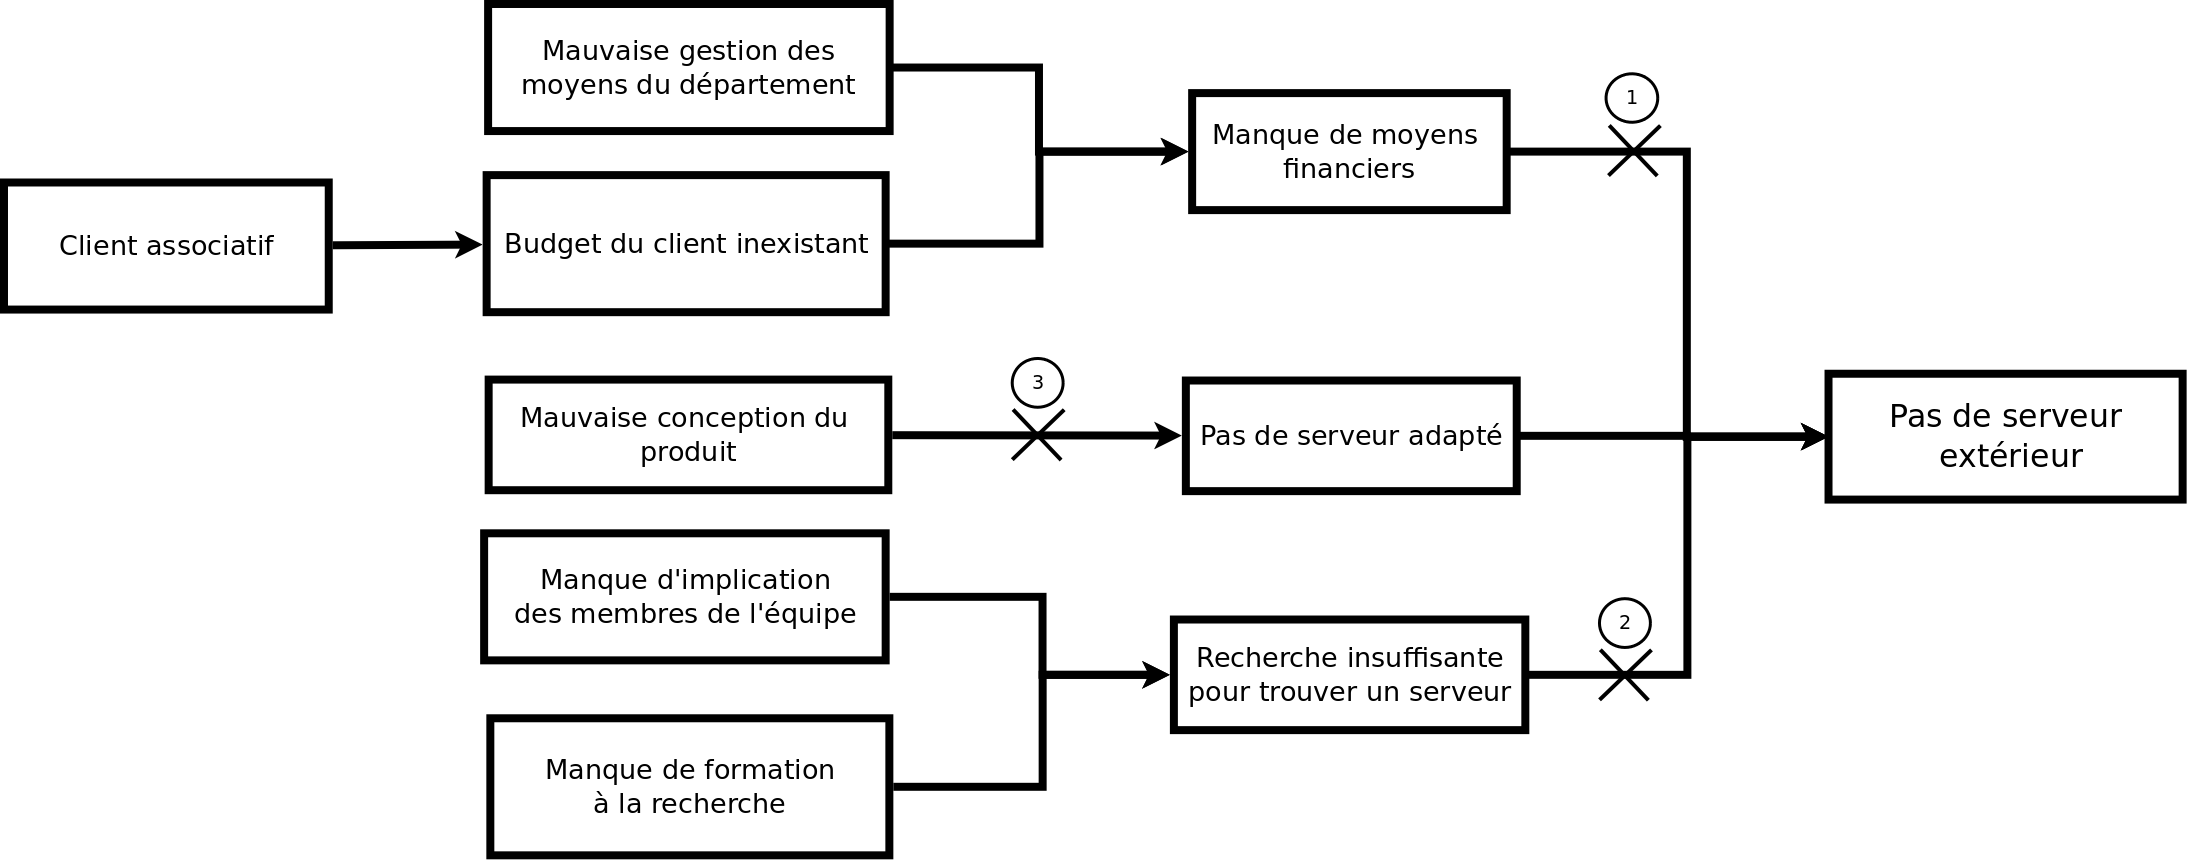
\includegraphics[scale=0.15]{images/AnalyseRisque_nPourquoi_FDR009}
	\caption{\label{risque pas de serveur ext}risque pas de serveur extérieur - méthode des n pourquoi}
\end{figure}
